\subsection{Bildegjenkjenning}

Gjenkjenning av objekter i bilder er en kompleks prosess. Ønsket i starten av dette prosjektet var å klare å gjenkjenne en bil i varierende terreng. 

For å opparbeide en forståelse for hvordan man gjenkjenning av bilder må man gjøre gjenkjenningsprosessen stegvis. Uten noen tidligere erfaring på området begynte vi med en enkel gemometrisk figur i en klar farge, for eksempel en gul ball, mot en svart bakgrunn med god belysning. En svart bakgrunn mot en klar farge er enkel å skille fra hverandre, og objektet trer lett frem slik at det kan behandles og en posisjon kan fastsettes. 

Dersom dette forsøket gjennomføres uten problemer kan man øke vanskelighetsgraden ved å utvide forsøket med en annen geometrisk figur, for eksempel en boks. En ny geometrisk figur medfører noen ekstra problemer. Forskjellen på en kule og en ball er at en kule er identisk uansett hvilken vinkel den betraktes fra, mens en boks vil variere ikke bare i fasong, men også kaste skygger, noe som fører til at fargen ikke er uniform over helt objektet. Utslaget fra dette er at gjenkjenningsalgoritmen må ta høyde for to nye faktorer; fargeulikhet og form.

Utforskningen kan deretter forsette ved å bevege objektet rundt i bildet, noe som fremhever fargeulikheten og gjør at objektet kan ha en ny fasong hele tiden. På dette stadiet kan man sammenligne bildegjenkjenningen med prosessering av video, der man må gjøre slik gjenkjenning for hver gang man får et bidle fra videokameraet. Her kreves det også at gjenkjenningen foregår relativt hurtig. 

Etter å ha testet kanskje andre genmetriske figurer på samme måte som med en boks, hvor hver nye flate eller ulikhet kan medføre nye problemer, kan man begynne å teste med noen réelle objekter. Vi forsøkte nå med en modell av en rød bil. Etter å ha finpusset gjenkjenningen med de andre geometriske modellene var ikke bilen noen stor utfordring. Vi prøvde dermed å fjerne det svarte bakteppet og teste mot diverse bakgrunner som vi kunne finne innendørs. Dette gjorde gjenkjenningen mye vanskeligere, da selv en klar rødfarge kan dukke opp delvis i objekter rundt i rommet. Når dette skjedde fikk vi mye støy inn i det behandlede bildet.

Bildebehandling er et komplisert fagfelt, og gjenkjenning av kompliserte objekter krever lang erfaring og en mengde arbeid som er urealistisk å kunne få til i den tiden vi har tigjengelig.

\subsection{Mekanisk Installasjon}
Når flyet skal svinge er flyet avhenigig av å gjøre en roll.
Dette fører til at buken til flyet ikke lengre peker rett ned mot bakken.
Et kamera i en låst posisjon, vil i denne situasjonen kunne oppleve at
objektet det skulle ha i bildet forsvinner ut av bildekanten.
Ved å feste kameraet til en mekanisk rigg som kan kompensesere for at flyet beveger
seg vil dette problemet kunne løses.

For å beskytte kameraet ble det bestemt at kameraet skal kunne
trekkes inn i flyet ved landing.
Siden målene på fullskala fly ikke er fremstilt fra Kongsberg ble det
bestemt å følge målene på modellen i presentasjonen sendt fra Kongsberg.
Denne viser at plassen inne i er maksimalt 10.5 cm i høyden og 7.2 cm i bredden.
Kravet for riggen ble dermed at den ikke kunne oppta større plass i bredde
og høyde enn dette med kameraet tilfestet.
Det ble antatt at det for modellens skyld kunne brukes et lite kamera,
på størrelse med et mobilkamera. Den andre grunnen til å bygge en liten rigg
er for å hindre at vekten blir for stor.
Kameraet må ha mulighet til å bevege synsretningen i x- og y-retning, noe som krever to servoer. Itilleg trengs en ekstra servomotor for å kunne trekke kameraet inn i flyet ved landing.

\subsubsection{Servomotor}
En servomotor er en inretning som kan rotere en arm til en bestemt vinkelposisjon og holde posisjonen.
Det finnes mange forskjellige servomotorer, med forskjellige egenskaper i forhold til nøyaktighet, kraft, pris, størrelse, vekt, kontrollsignaler, motortyper og kildespenning. 
Enkle servomotorer kan bestå av enkle DC motorer med børster og kan bare justere posisjons mellom -90 til +90 grader fra senter, mens avanserte servoer kan ha børsteløse motorer og ha mulighet til full rotasjon, med kontrollbar vinkelhastighet og tilbakemelid av posisjon og fart. 
En servomotor er bygget opp av en elektrisk motor, en vinkelsensor og en kontroll enhet.
Et kommandosignal, som representere en vinkelposisjon, påtrykkes inngangen, dette fører til at motoren roterer i retning av denne posisjonen. Vinkelsensoren registrer hele tiden posisjonen til armen og kontrollenheten sammenlikner denne med den ønskede posisjonen. Når den ønskede vinkelposisjonen er nådd stopper motoren. Hvis armen skyves bort fra denne posisjonen vil kontrollenheten registere at den nåværende vinkelen avviker fra ønsket vinkel og motoren vil flytte armen tilbake i rett posisjon.

I dette prosjektet ble det brukt servomotorer av typen HD-1600A fra PowerHD [\ref{ref:PowerHD}]. Dette er en enkel analog servomotor, beregnet for radiostyrte modellfly, som består av en DC motor, en potensiometer som vinkelsensor og en kontrollenhet av typen YT2462B. For å kontrollere denne typen servomotorer brukes puls-bredde-modulasjon (PWM). I PWM sendes firkantpulser hvor pulslengden varieres, mens grunnfrekvensen holdes konstant. Informasjonen ligger dermed i lengden av pulsen. For styring av analoge RC servoer som HD-1600A er det vanlig å bruke en grunnfrekvens på 50Hz og bulsbredde på 1ms til 2ms [\ref{ref:SerCtrl}]. Figur \ref{fig:PWM} viser hvordan servovinkel avhenger av pulsbredde.

<<<<<<< HEAD
En servomotor er en inretning som lar en kontrolere og holde på en vinkelposisjon.
En servomotor er bygget opp av en elektrisk motor,
en vinkelsensor og en kontroll enhet.
Et signal påtrykkes inngangen og motoren begynner å gå.
Vinkelsensoren vil fortelle vinkelen og når vinkelen som koresponderer
til inngangssignalet er nådd vil motoren stoppe.
Vinkelsensoren oppfører seg derfor som en tilbakekobling som returenerer feilen

\subsection{Hardware}
For å kunne styre riggen er det nødvendig å ha en datamaskin ombord i flyet. Det finnes en rekke alternativer på dette området, men her vil Arduino og Raspberry Pi bli presantert. Hovedoppgaven til datamskinen blir å få data fra kameraet, og orientere riggen etter disse. I systemspesifikasjonene til Kongsberg blir presisert at det allerede finnes en ekstern GPU som tar av seg bildebehandling, men man kan også tenke seg en løsning for all funksjonalitet er samlet på en chip. Datamaskinen må også kunne håndtere flere prosessorer uten at det blir konflikt mellom dem. 

\paragraph{Arduino}
Arduino er en open-source utviklings platform basert på 8bit \textit{atMega328}. Bruksområdet er hovedsakelig mindre prosjekter. Kortet har 14 digtale porter, samt 6 analoge in-porter. 6 av de digitale portene kan sende PWM-signaler. Servomotorer bruker disse signalene, og det er derfor mulig å koble opp til 6 servoer til Arduino. 
\begin{figure}[h!]
\centering
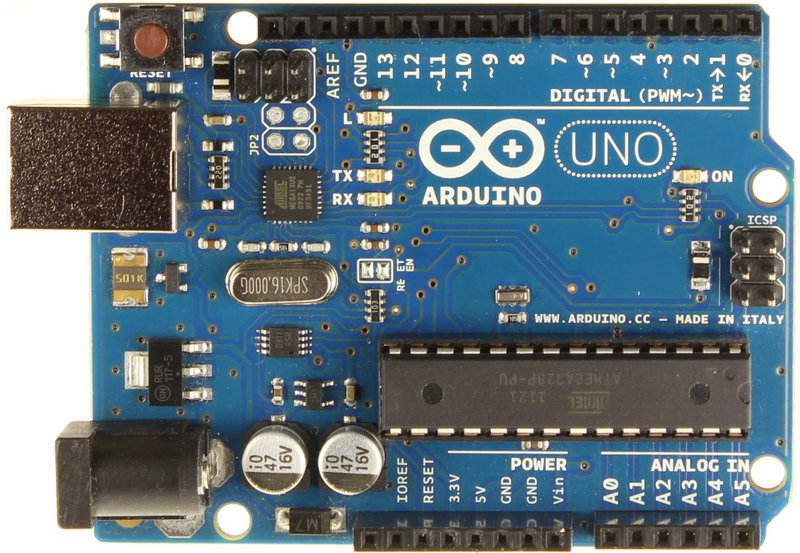
\includegraphics[scale = 0.25]{img/arduinoBoard.jpg}
\caption{Arduino Uno R3}
\end{figure}
Arduino programmeres i C++, og programmene overføres til kortet via USB. USB-porten på kortet kan også benyttes som COM-port slik at Arduinoen kan ta inn eksterne kommandoer. Disse kommandoen kan for eksempel være vinkler som servomotorer skal innstilles til. På mikrokontrolleren er det også innstallert en bootlader som inneholder en rekke bilbioteker som gjør at abstraksjonsnivået blir høyere enn generell AVR-programmering. Dataregistre trenger ikke å endres når man vil åpne opp for en funksjon fordi bilibioteket vil håndtere dette. 

\paragraph{Raspberry Pi}
Raspberry Pi er en datamskin basert på 32-bit ARM-arkitektur. Linux er innstalert på et SD-kort, og all programmering skjer direkte på Raspberry PI. Den kan brukes ved å koble den til en monitor via HDMI, eller man kan koble den til internett via ethetnet-porten og bruke ssh fra en annen datamaskin. Kortet har 8 i/o pins, pinner som kan brukes til seriell kommunikasjon. Den er også utstyrt med 2 usb-porter.  

\begin{table}[h!]
\caption{Sammenligning mellom Arduino og Raspberry Pi}
\centering
\begin{tabular}{ |c |c |c| }
	\hline
   & Arduino & Raspberry Pi \\
	\hline
  CPU & 	ATmega328 & ARM1176JZF-S \\
  Klokkehastighet & 16 MHz & 700 MHz \\
	Minne & 32KB & 512MB\\ 
	CPU-størrelse & 8bit & 32bit\\
	i/o-porter & 14 & 8 \\
	PWN-porter & 6 & 1 \\
	USB-porter & 1 & 2 \\
	Strømforbruk & 250mW & 3.5W\\
	Pris & \$26 & \$35 \\
	\hline  
\end{tabular}
\end{table}



=======
\begin{figure}[H]
\centering
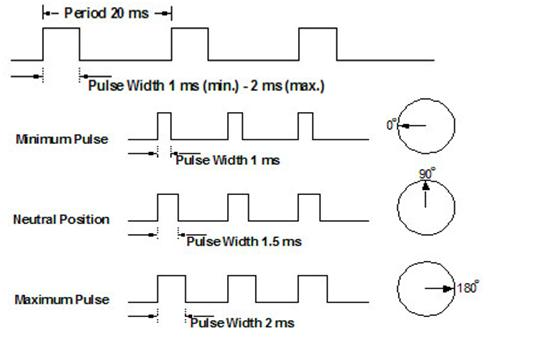
\includegraphics[width=0.8\textwidth]{img/pwm_servo.jpg}
\caption{PWM servo kontrollsignal}
\label{fig:PWM}
\end{figure}   
>>>>>>> 5f20608936041630d150b0ca519f96a0d724648d
